

\documentclass[12pt]{article}%
\usepackage{amsmath}%

%\usepackage{bibentry}%
\usepackage{amsfonts}%
\usepackage{amssymb}%
\usepackage{setspace}%
\usepackage{bbm}%
%\usepackage{harvard}
%\usepackage{chicago}
%\bibpunct[,~]{(}{)}{;}{a}{}{,}
\usepackage{enumerate}%
\usepackage{xfrac}
\usepackage[top=1in, bottom=1in, left=1in, right=1in]{geometry}
\usepackage{multirow}
\usepackage{rotating,graphicx}
\usepackage{subcaption}
\usepackage{caption}
\usepackage{rotating}
\usepackage{booktabs}
\usepackage[flushleft]{threeparttable}
\usepackage{subcaption}
\usepackage{float}
\usepackage{appendix}
\usepackage{titletoc}
\usepackage{rotating}



\usepackage[bookmarks=false,colorlinks=true, linkcolor=black, urlcolor=black, citecolor=black]{hyperref}

\usepackage{fullpage}

\usepackage{titlesec}

\usepackage[comma,longnamesfirst]{natbib}%

\newtheorem{hypothesis}{Hypothesis}
\usepackage{xcolor}

\usepackage{xr}

\pdfminorversion=6
\bibpunct[,~]{(}{)}{;}{a}{}{,}
\bibliographystyle{apsr}

\begin{document}
	
	\pagenumbering{arabic}
	\begin{doublespace}


\section*{Appendix A - Robustness}
This appendix presents a series of robustness checks for the main results reported in the main body of the paper.

\subsection*{Subsample Analyses}
The main body of the paper reports results from a pooled sample made up of a nationally representative sample and a low-socioeconomic status oversample in order to preserve statistical power. This appendix reports the main results of the paper for each subsample.

\begin{figure}[h!]
	\centering
	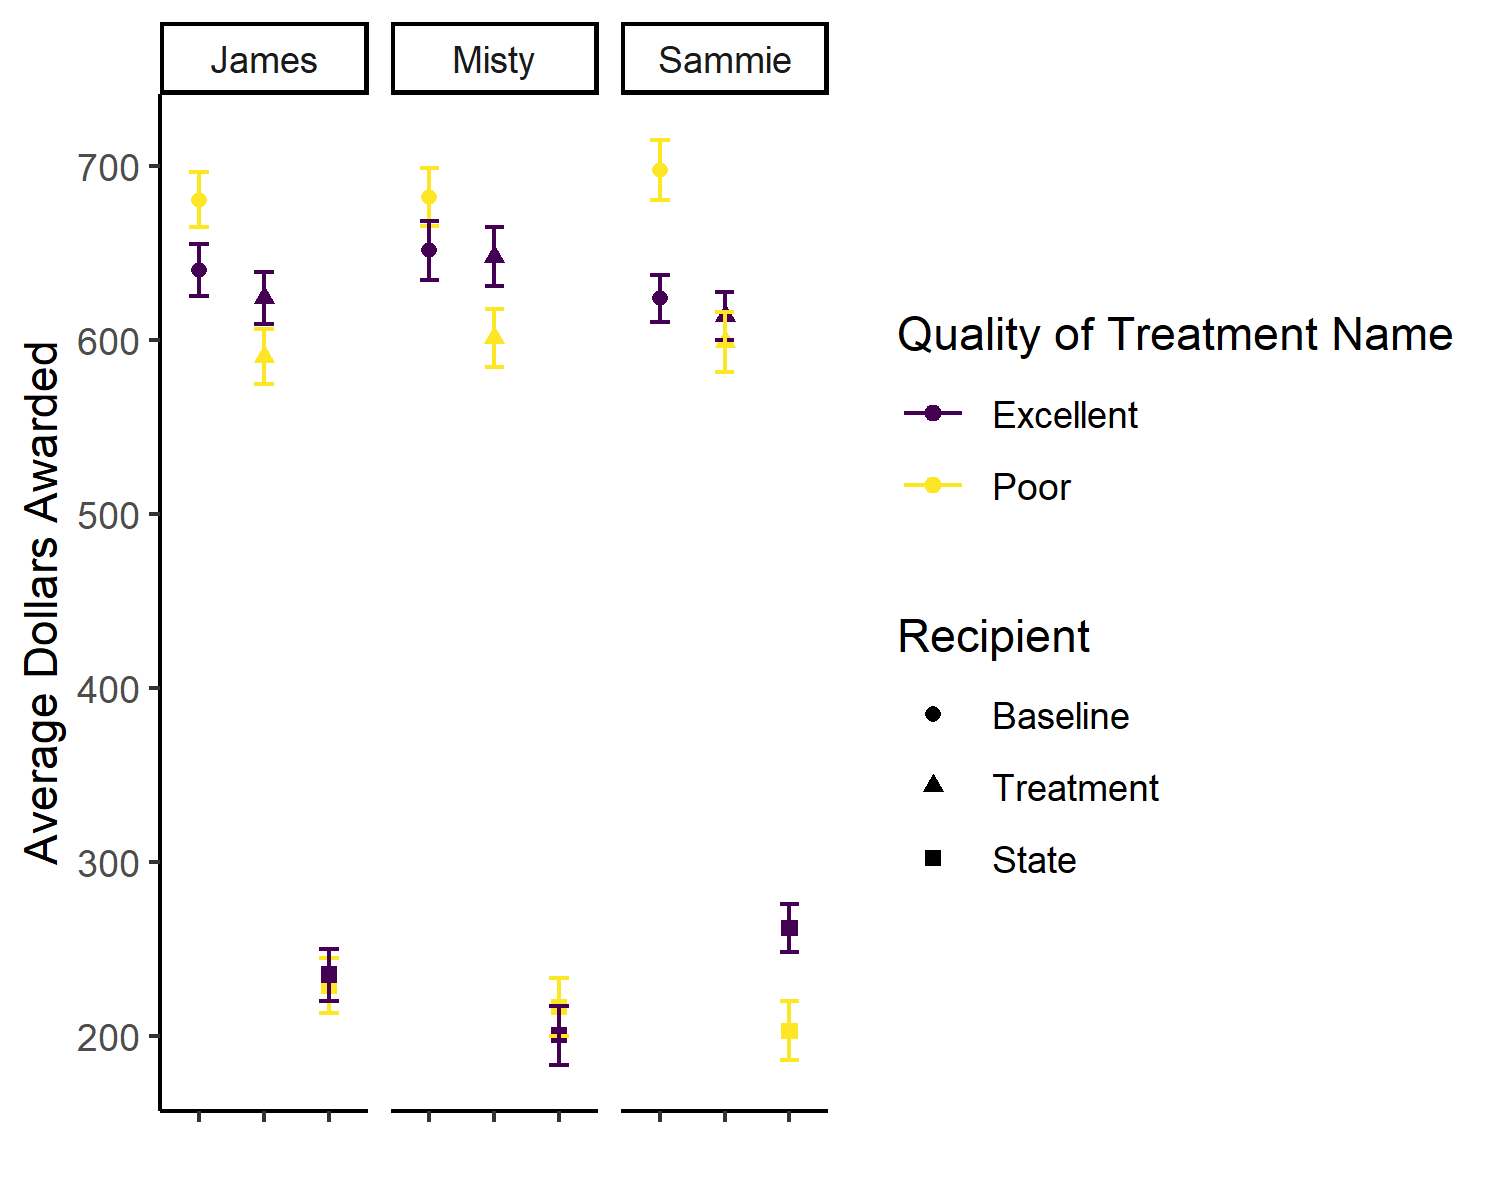
\includegraphics[scale=1]{figs/results-gen-pop.png}
	\caption{Results Restricted to Nationally Representative Subsample}
	\label{}
\end{figure}

Restricting the sample to the nationally representative subsample, I find that male names are still awarded less relative to the baseline than female names, but this difference is not statistically significant at conventional levels.

% Date and time: Wed, Feb 22, 2023 - 11:57:15 AM
\begin{table}[!htbp] \centering 
	\caption{Testing H1 with Nationally Representative Sample} 
	\label{} 
	\footnotesize 
	\begin{tabular}{@{\extracolsep{1pt}} cccccc} 
		\\[-1.8ex]\hline \\[-1.8ex] 
		& Condition & Mean Difference & Upper CI & Lower CI & p-value \\ 
		\hline \\[-1.8ex] 
		& Excellent Misty vs Baseline & 3.537 & -11.467 & 18.542 & 0.643 \\ 
		& Excellent James vs Baseline & 16.065 & -8.571 & 40.7 & 0.2 \\ 
		& Excellent Sammie vs Baseline & 10.041 & -7.728 & 27.81 & 0.266 \\ 
		\hline \\[-1.8ex] 
	\end{tabular} 
\end{table} 

I find that Excellent Misty is awarded more than Poor Misty and that these differences are statistically significant at conventional levels, whereas the difference in means between Poor and Excellent James and Poor and Excellent Sammie are not statistically significant at conventional levels.

\begin{table}[!htbp] \centering 
	\caption{} 
	\label{} 
	\footnotesize 
	\begin{tabular}{@{\extracolsep{1pt}} ccccccc} 
		\\[-1.8ex]\hline \\[-1.8ex] 
		& Condition & Mean 1 & Mean 2 & Upper CI & Lower CI & p-value \\ 
		\hline \\[-1.8ex] 
		& Excellent Misty vs Poor Misty & 648.09 & 601.396 & 7.527 & 85.86 & 0.02** \\ 
		& Excellent James vs Poor James & 624.393 & 590.662 & -7.489 & 74.952 & 0.108 \\ 
		& Excellent Sammie vs Poor Sammie & 614.041 & 599.09 & -28.278 & 58.181 & 0.497 \\ 
		\hline \\[-1.8ex] 
	\end{tabular} 
\end{table} 



\begin{figure}[h!]
	\centering
	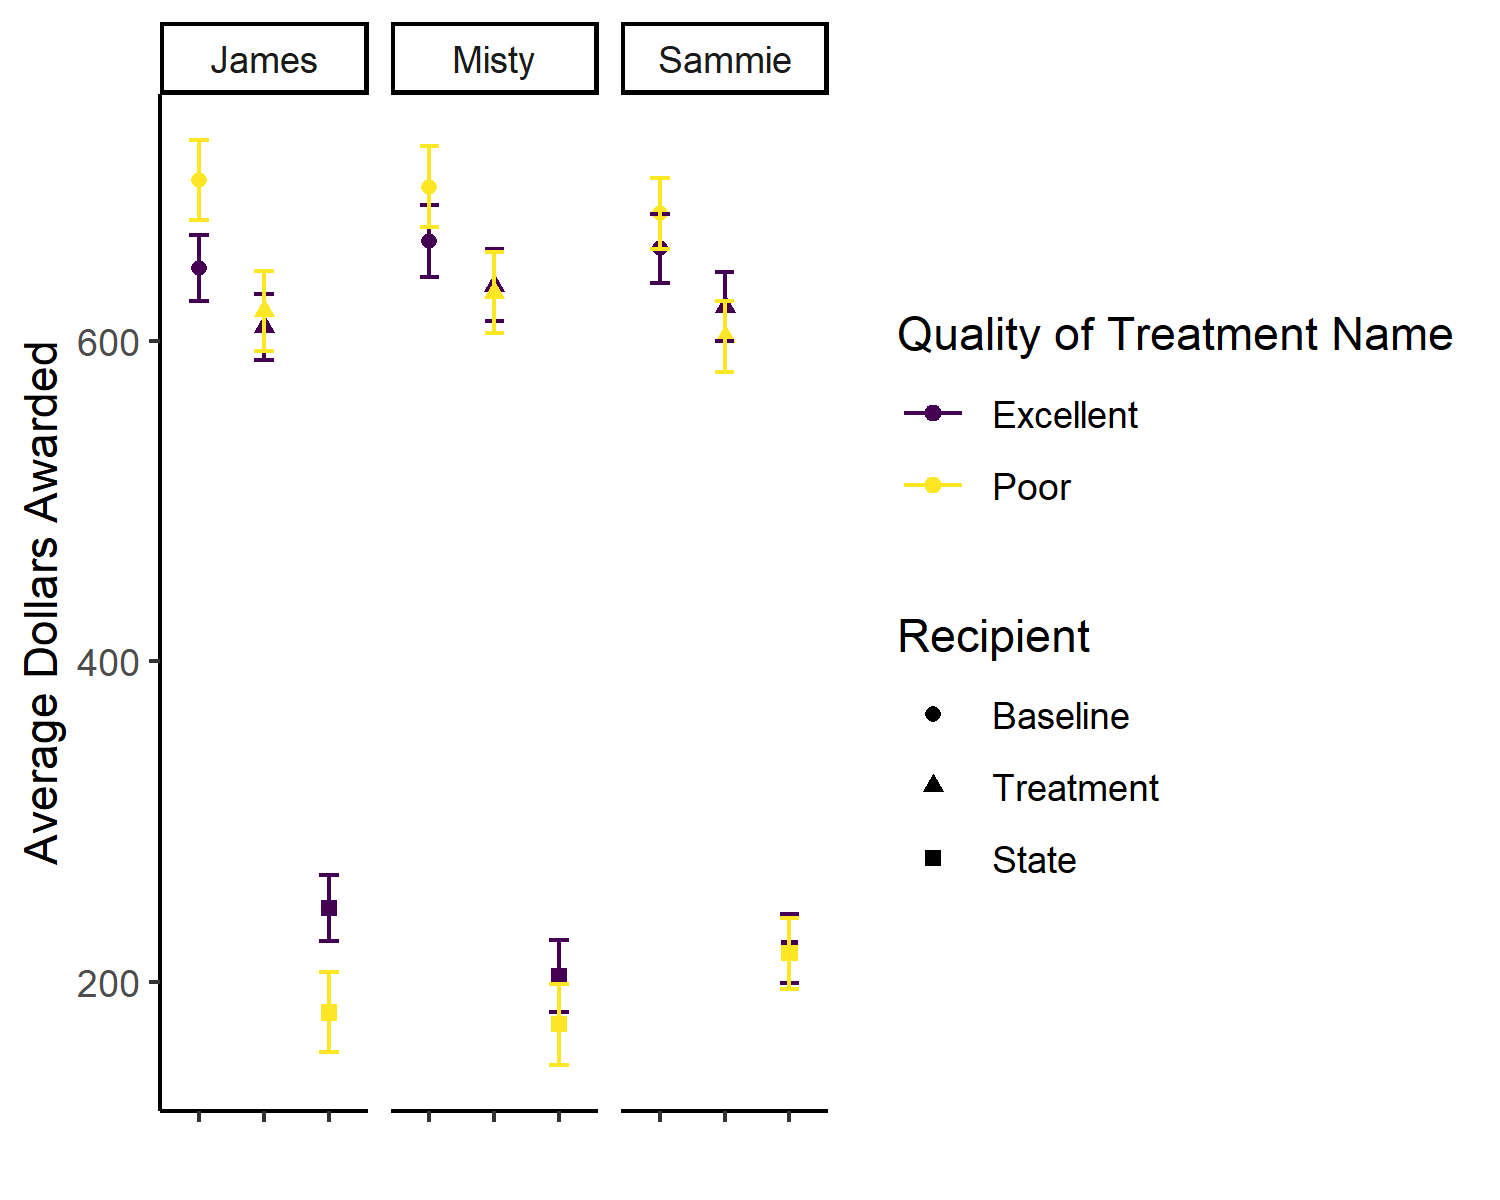
\includegraphics[scale=.75]{figs/results-low-ses.png}
	\caption{Results Restricted to Low SES Subsample}
	\label{}
\end{figure}


Restricting the analysis to the low SES subsample, I find that many of my results on the full sample hold. The amount awarded to Excellent Misty is statistically indistinguishable from the amount awarded to the baseline. Excellent James earns significantly less than the baseline, as does Excellent Sammie.


% Table created by stargazer v.5.2.3 by Marek Hlavac, Social Policy Institute. E-mail: marek.hlavac at gmail.com
% Date and time: Wed, Feb 22, 2023 - 11:51:22 AM
\begin{table}[!htbp] \centering 
	\caption{Testing H1 with Low SES Subsample} 
	\label{} 
	\footnotesize 
	\begin{tabular}{@{\extracolsep{1pt}} cccccc} 
		\\[-1.8ex]\hline \\[-1.8ex] 
		& Condition & Mean Difference & Upper CI & Lower CI & p-value \\ 
		\hline \\[-1.8ex] 
		 & Excellent Misty vs Baseline & 27.491 & -9.06 & 64.042 & 0.139 \\ 
		 & Excellent James vs Baseline & 36.948 & 12.719 & 61.178 & 0.003*** \\ 
		 & Excellent Sammie vs Baseline & 36.318 & 8.942 & 63.694 & 0.01** \\ 
		\hline \\[-1.8ex] 
	\end{tabular} 
\end{table} 

However, Excellent Misty earns only \$4 more on average than Poor Misty and this difference is not statistically significant. Excellent James earns \textit{less} than Poor James on average, but this difference is not statistically significant either. Excellent Sammie earns more than Poor Sammie, but this difference is also not statistically significant.

\begin{table}[!htbp] \centering 
	\caption{Testing H3a-b with Low SES Subsample} 
	\label{} 
	\footnotesize 
	\begin{tabular}{@{\extracolsep{1pt}} ccccccc} 
		\\[-1.8ex]\hline \\[-1.8ex] 
		& Condition & Mean 1 & Mean 2 & Upper CI & Lower CI & p-value \\ 
		\hline \\[-1.8ex] 
		 & Excellent Misty vs Poor Misty & 634.42 & 630.119 & -45.183 & 53.783 & 0.864 \\ 
		 & Excellent James vs Poor James & 608.433 & 618.682 & -61.091 & 40.592 & 0.691 \\ 
		 & Excellent Sammie vs Poor Sammie & 621.234 & 602.602 & -38.23 & 75.494 & 0.519 \\ 
		\hline \\[-1.8ex] 
	\end{tabular} 
\end{table} 

These results suggest one of two things. First, it is possible that the treatments effect the two subsamples differently. Perhaps the general population cares more about applicant quality and less about gender, whereas low income populations bring stronger gender stereotypes into deservingness evaluations. However, another consideration is that these differences in results are an artifact of randomization because I randomized treatments over the whole sample, not over the two subsamples individually.


\section*{Appendix C - Survey Questions}
Subjects were shown two applicants for state aid with the following prompt:

``Researchers have been hired to consult with a nearby state’s welfare agency. Below you will find two applicants for government assistance. The application information has been redacted to hide information that may identify individual applicants.

Each applicant has a state-assessed level of need of \$900 per month. \textbf{Your task is to allocate \$1,500 between the two applicants. You can allocate any amount between \$0 and \$900 to each applicant. Any remaining funds will be used to offset the state’s budget deficit.}"

Respondents were given three sliding scales to allocate funds. They could slide the bars or type numbers into the boxes on the right. At the bottom of the screen, the total amount they had awarded was shown relative to the full \$1,500 they had to distribute.

\begin{figure}[h!]
	\centering
	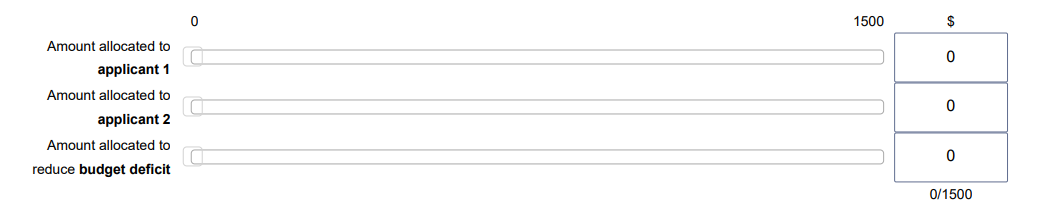
\includegraphics[scale=1]{figs/sliding-scale.png}
	\caption{Sliding Scale Used by Respondents to Make Allocations}
	\label{}
\end{figure}




\end{doublespace}

\end{document}




